\documentclass[a4paper,class=article,border=10pt,tikz]{standalone}
\usepackage{tikz}
\usetikzlibrary{snakes,calc,positioning,patterns,angles,quotes,decorations.pathmorphing,decorations.markings,through}
\usetikzlibrary{arrows,decorations,decorations.text}
\usepackage{rotating}
\usetikzlibrary{arrows,decorations,decorations.text}
\usetikzlibrary{patterns.meta,math}




\usepackage{siunitx}

\begin{document}

 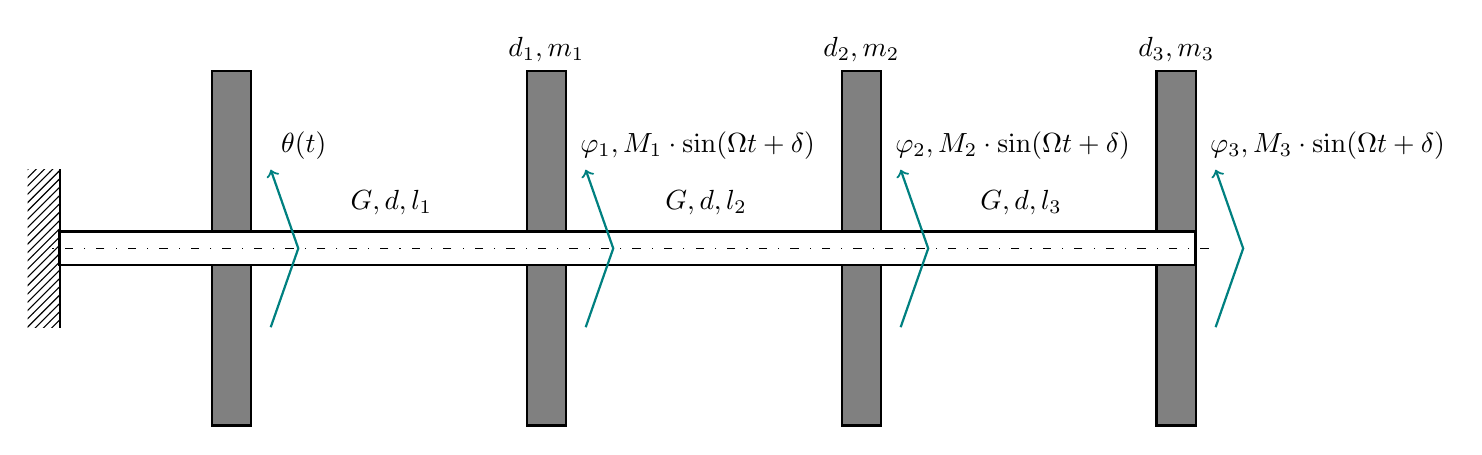
\begin{tikzpicture}

    \tikzstyle{ground}=[fill,pattern=north east lines,draw=none,minimum width=0.75cm,minimum height=0.3cm]
     \tikzstyle{close}=[draw=none,minimum width=0.75cm,minimum height=0.3cm]
      \coordinate (origo) at (0,0);

\node (I_3) [fill=gray,draw,outer sep=0pt,thick,minimum width=0.5cm,xshift=-0.03cm, minimum height=4.5cm,label=above:{$d_3,m_3$}]  at (origo) {};
\node (I_2) [fill=gray,draw,outer sep=0pt,thick,minimum width=0.5cm, minimum height=4.5cm,xshift=-4cm,label=above:{$d_2,m_2$}]  at (I_3) {};
\node (I_1) [fill=gray,draw,outer sep=0pt,thick,minimum width=0.5cm, minimum height=4.5cm,xshift=-4cm,label=above:{$d_1,m_1$}]  at (I_2) {};
\node (I_0) [fill=gray,draw,outer sep=0pt,thick,minimum width=0.5cm, minimum height=4.5cm,xshift=-4cm]  at (I_1) {};




\draw[thick,double=white,double distance=0.4cm,line cap=rect] (origo) node (start){} --++(-2cm,0) node[xshift=0cm,above=+0.3cm] (Label1){$G,d,l_3$} -- ++ (0cm,0) node (P_load){} -- ++ (-5.5cm,0) node[xshift=1.5cm,above=+0.3cm] (Label2){$G,d,l_2$} -- ++ (-6.5cm,0) node (shaft_end){} node[xshift=4cm,above=+0.3cm] (Label3){$G,d,l_1$} -- ++ (0,0) node (shaft_end){};

\draw [thin, loosely dashdotted] ([xshift=0.25cm]start.east) --([xshift=-0.25cm]shaft_end.west);

\node (wall_1) [ground,anchor=east,xshift=-14.21cm,yshift=0cm,minimum height=2cm ,minimum width=0.4cm] at (origo) {};

\draw[thick] (wall_1.north east) -- (wall_1.south east);

\draw[thick, teal,->] (I_0)++(0.5cm,-1cm)  --++(0.35cm,1cm) --++ (-0.35cm,1cm) node[above right, black] {$\theta(t)$};

\draw[thick, teal,->] (I_1)++(0.5cm,-1cm)  --++(0.35cm,1cm) --++ (-0.35cm,1cm) node[above right,xshift=-0.2cm, black] {$\varphi_1,{M_{1}} \cdot{\sin({\Omega}{t}+{\delta})}$};

\draw[thick, teal,->] (I_2)++(0.5cm,-1cm)  --++(0.35cm,1cm) --++ (-0.35cm,1cm) node[above right,xshift=-0.2cm, black] {$\varphi_2,{M_{2}} \cdot{\sin({\Omega}{t}+{\delta})}$};

\draw[thick, teal,->] (I_3)++(0.5cm,-1cm)  --++(0.35cm,1cm) --++ (-0.35cm,1cm) node[above right,xshift=-0.2cm, black] {$\varphi_3,{M_{3}} \cdot{\sin({\Omega}{t}+{\delta})}$};

\end{tikzpicture}


\end{document}